\section{Justificación de la arquitectura distribuida}

\subsection{Por qué el problema exige distribuir el sistema}

El sistema atiende a tres grupos de usuarios que no comparten lugar ni horario: clientes que
reportan una falla, agentes de mesa de ayuda y técnicos de campo que actualizan el estado desde el
celular. El servicio se usa todos los días y el SLA se mide en horas, de modo que una caída no es
un inconveniente: es un incumplimiento contractual con costo medible
(tabla~\ref{tab:consecuencias}).

Tres requisitos no funcionales sostienen la decisión. El \textbf{RNF-01} exige 99,5\,\% de
disponibilidad mensual, es decir, un máximo de 3,6 h fuera de servicio: eso obliga a tener más de
una instancia y a que un fallo no arrastre a todo el sistema. El \textbf{RNF-02} exige que el alta
de la incidencia funcione aunque el servicio de adjuntos esté caído: eso obliga a separar
responsabilidades y a tolerar fallos parciales. El \textbf{RNF-04} exige sostener 200 usuarios
concurrentes en el pico posterior a un corte sin degradar la latencia: eso obliga a escalar solo la
parte que recibe la carga, no el sistema completo.

\subsection{Por qué no basta un sistema monolítico}

Un monolito en un único servidor incumple los tres requisitos anteriores por construcción. La
disponibilidad queda limitada por un solo proceso y un solo equipo: si el despliegue falla, el
servicio completo se detiene. Es exactamente el riesgo \textbf{R-02} documentado en FORM-AC-01, y
el incidente de Fastly~\cite{fastly2021} muestra la magnitud del problema: un cambio de
configuración válido dejó al 85\,\% de la red devolviendo errores, y el equipo tardó 40 minutos en
identificar la configuración culpable. En SGIRI, una sola instancia significa el 100\,\% del
servicio caído y sin segunda copia para comparar.

La escalabilidad tampoco se resuelve replicando el monolito completo, porque el pico de carga se
concentra en el registro y la asignación de incidencias, no en la generación de reportes. Replicar
todo para escalar una parte multiplica el costo y no reduce el acoplamiento.

La mantenibilidad es el tercer límite: el RNF-06 exige desplegar notificaciones sin detener
incidencias. Con un despliegue conjunto, cada cambio en un módulo obliga a detener los demás, y cada
detención consume el presupuesto de disponibilidad del RNF-01.

\subsection{Qué se distribuye y qué no}

Distribuir no es fragmentar todo. En este proyecto se distribuye lo que tiene ritmos distintos de
cambio y de carga (incidencias, técnicos, notificaciones, identidad), y se mantiene junto lo que
debe ser consistente en una sola operación (estado y asignación del ticket). El análisis
CAP/PACELC de la sección~\ref{sec:cap} fija esa frontera dato por dato.

\section{Arquitectura base con el modelo C4}

\subsection{Nivel 1: contexto}

\begin{figure}[H]
\centering
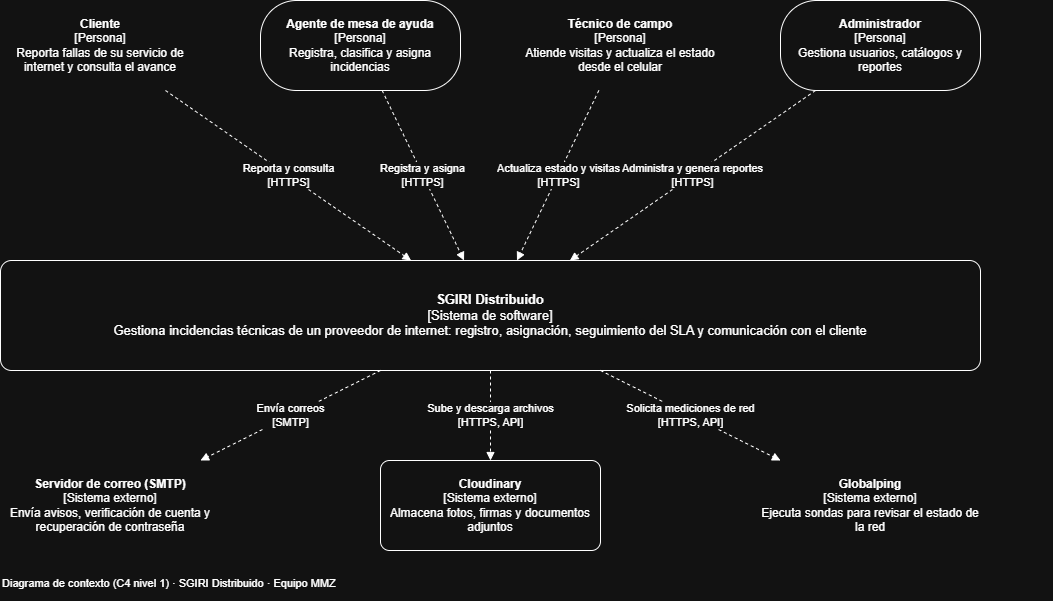
\includegraphics[width=\textwidth]{diagramas/C4-nivel-1-SGIRI.png}
\caption{Diagrama de contexto de SGIRI Distribuido (nivel 1 del modelo C4).}
\label{fig:c4n1}
\end{figure}

\subsection{Nivel 2: contenedores}

\begin{figure}[H]
\centering
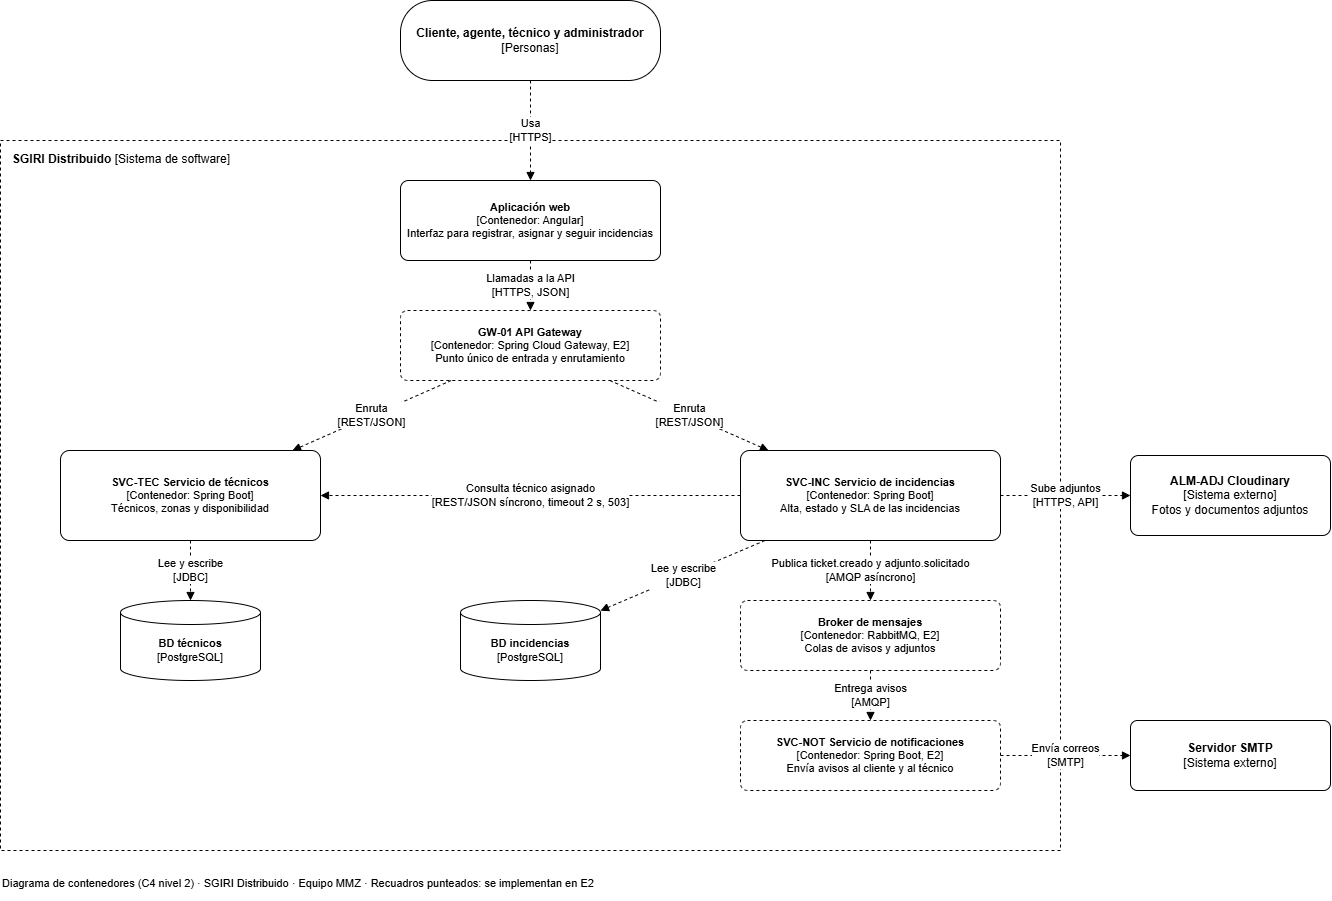
\includegraphics[width=\textwidth]{diagramas/C4-nivel-2-SGIRI.png}
\caption{Diagrama de contenedores: servicios, bases de datos y comunicación (nivel 2 del modelo C4).}
\label{fig:c4n2}
\end{figure}

\section{Modelo de comunicación entre servicios}
\label{sec:comunicacion}

Cada interacción del diagrama de contenedores se clasifica por tipo (sincrónica o asincrónica),
mecanismo (REST, gRPC, mensajería) y la razón por la que se eligió, apoyada en lo medido en PE-U1
y en lo decidido en el ADR-002. Los identificadores son los mismos del diagrama de contenedores:
\texttt{SVC-INC} (incidencias), \texttt{SVC-TEC} (técnicos), \texttt{SVC-NOT} (notificaciones),
\texttt{GW-01} (API Gateway) y \texttt{ALM-ADJ} (almacenamiento de adjuntos).

\begin{longtable}{@{}p{2.5cm} p{1.9cm} p{1.9cm} p{3.9cm} p{3.9cm}@{}}
\caption{Interacciones entre contenedores}
\label{tab:comunicacion}\\
\toprule
Interacción & Tipo & Mecanismo & Justificación & Tolerancia a fallos \\
\midrule
\endfirsthead
\toprule
Interacción & Tipo & Mecanismo & Justificación & Tolerancia a fallos \\
\midrule
\endhead
\bottomrule
\endfoot
\texttt{SVC-INC} $\rightarrow$ \texttt{SVC-TEC}
& Sincrónica & REST/JSON & El agente espera la respuesta para asignar; el dato cambia poco y se
consulta con frecuencia & \emph{Timeout} 2 s, 2 reintentos, \texttt{503} controlado \\
\addlinespace
\texttt{SVC-INC} $\rightarrow$ \texttt{SVC-NOT}
& Asincrónica & Mensajería (AMQP) & El aviso no debe bloquear el alta; si falla, se reintenta sin
perder el ticket & Cola con reintento y cola de fallos \\
\addlinespace
\texttt{SVC-INC} $\rightarrow$ \texttt{ALM-ADJ}
& Asincrónica & Mensajería (AMQP) & Mitiga el riesgo R-03: el ticket se registra primero y el
adjunto se sube después & Reintento con límite; estado «adjunto pendiente» \\
\addlinespace
Cliente $\rightarrow$ \texttt{GW-01} $\rightarrow$ servicios
& Sincrónica & REST/JSON & Punto único de entrada, autenticación y límites de tasa & Gateway con
verificación de salud \\
\end{longtable}

\section{Análisis CAP y PACELC}
\label{sec:cap}

El teorema CAP describe qué se sacrifica durante una partición de red~\cite{gilbert2012}; PACELC
agrega qué se sacrifica cuando no la hay~\cite{abadi2012}. La tabla se lee por dato crítico, no por
servicio.

\begin{longtable}{@{}p{3.3cm} p{4.3cm} p{3.9cm} p{3.5cm}@{}}
\caption{Decisión CAP/PACELC por dato crítico}
\label{tab:cap}\\
\toprule
Dato crítico & En partición (CAP) & Sin partición (PACELC) & Consecuencia para el usuario \\
\midrule
\endfirsthead
\toprule
Dato crítico & En partición (CAP) & Sin partición (PACELC) & Consecuencia para el usuario \\
\midrule
\endhead
\bottomrule
\endfoot
Estado del ticket & \textbf{CP}: se rechaza la escritura antes que aceptar un estado dudoso &
\textbf{EC}: se espera la confirmación antes de responder &
El técnico ve un error y reintenta; nunca ve un ticket «resuelto» que en realidad no lo está (RNF-02) \\
\addlinespace
Asignación al técnico & \textbf{CP}: no se asigna sin confirmación del servicio de técnicos &
\textbf{EC}: consistencia antes que latencia &
Si el servicio de técnicos no responde, el agente puede guardar el ticket como «sin asignar» y
asignarlo después; no se pierde el caso (RNF-02) \\
\addlinespace
Notificaciones y adjuntos & \textbf{AP}: se acepta el evento y se entrega cuando la red vuelva &
\textbf{EL}: latencia antes que consistencia &
El cliente recibe el aviso con retraso, pero el ticket ya existe (RNF-02, RNF-06) \\
\addlinespace
Consulta de disponibilidad de técnicos & \textbf{AP}: se responde con la última copia conocida &
\textbf{EL} &
El agente puede ver una disponibilidad desactualizada por segundos; el sistema lo advierte (RNF-03) \\
\addlinespace
Auditoría de cambios & \textbf{AP}: se registra localmente y se replica después &
\textbf{EL} &
Ninguna operación se pierde del registro aunque el nodo de auditoría esté caído (RNF-01) \\
\end{longtable}

\section{Registros de decisiones de arquitectura}

Los ADR completos están en \texttt{docs/adr/} y se versionan con el repositorio.

\begin{table}[H]
\centering
\caption{Resumen de los ADR}
\label{tab:adr}
\small
\begin{tabularx}{\linewidth}{@{}lYY@{}}
\toprule
ADR & Decisión & Consecuencia principal \\
\midrule
ADR-001 & Microservicios por dominio con API Gateway, sin orquestación compleja &
Despliegue independiente y aislamiento de fallos, a cambio de complejidad operativa que se acota a
cinco servicios \\
\addlinespace
ADR-002 & REST/JSON síncrono para consultas y mensajería asíncrona para notificaciones y adjuntos &
Consultas predecibles; el alta no depende de servicios externos \\
\bottomrule
\end{tabularx}
\end{table}

\section{Riesgos}
\label{sec:riesgos}

Los tres primeros riesgos provienen del análisis de FORM-AC-01 (incidente de Fastly del 8 de junio
de 2021, \cite{fastly2021}) aplicado a SGIRI; los dos restantes son propios de este proyecto.

\begin{longtable}{@{}p{0.8cm} p{4.6cm} p{1.0cm} p{1.1cm} p{5.9cm}@{}}
\caption{Riesgos técnicos, probabilidad, impacto y mitigación}
\label{tab:riesgos}\\
\toprule
ID & Riesgo & Prob. & Impacto & Medida de mitigación verificable \\
\midrule
\endfirsthead
\toprule
ID & Riesgo & Prob. & Impacto & Medida de mitigación verificable \\
\midrule
\endhead
\bottomrule
\endfoot
R-01 & Un cambio válido en las reglas de transición deja el ticket sin salida y con el SLA
corriendo & Media & Alto & Validar la máquina de estados; transición inválida devuelve \texttt{409}
sin alterar estado ni contador; pruebas de todas las transiciones \\
\addlinespace
R-02 & Un despliegue con credencial o URL mal configurada no arranca y, con una sola instancia,
detiene todo el servicio & Media & Muy alto & Dos instancias con verificación de salud antes de
recibir tráfico; conservar artefacto anterior; arranque verificado en entorno de prueba \\
\addlinespace
R-03 & El alta de la incidencia depende de un servicio externo de adjuntos y termina en error 500 &
Alta & Alto & Registrar el ticket primero y subir después, con tiempo límite y reintento; prueba con
el servicio externo bloqueado \\
\addlinespace
R-04 & \pendiente{riesgo propio: por ejemplo, coherencia de datos entre el ticket y el técnico
asignado} & \pd & \pd & \pendiente{} \\
\addlinespace
R-05 & \pendiente{riesgo propio: por ejemplo, dependencia de la conectividad del local del cliente}
& \pd & \pd & \pendiente{} \\
\end{longtable}
